% Pipeline figure of the UDIVA-HHOI Track-2 entry (Team JLShen) -- same figure as Fig. 1 of
% the fact sheet. Build with: pdflatex pipeline.tex
\documentclass[border=6pt]{standalone}
\usepackage{amsmath}
\usepackage{amssymb}
\usepackage{tikz}
\usetikzlibrary{arrows.meta}
\begin{document}
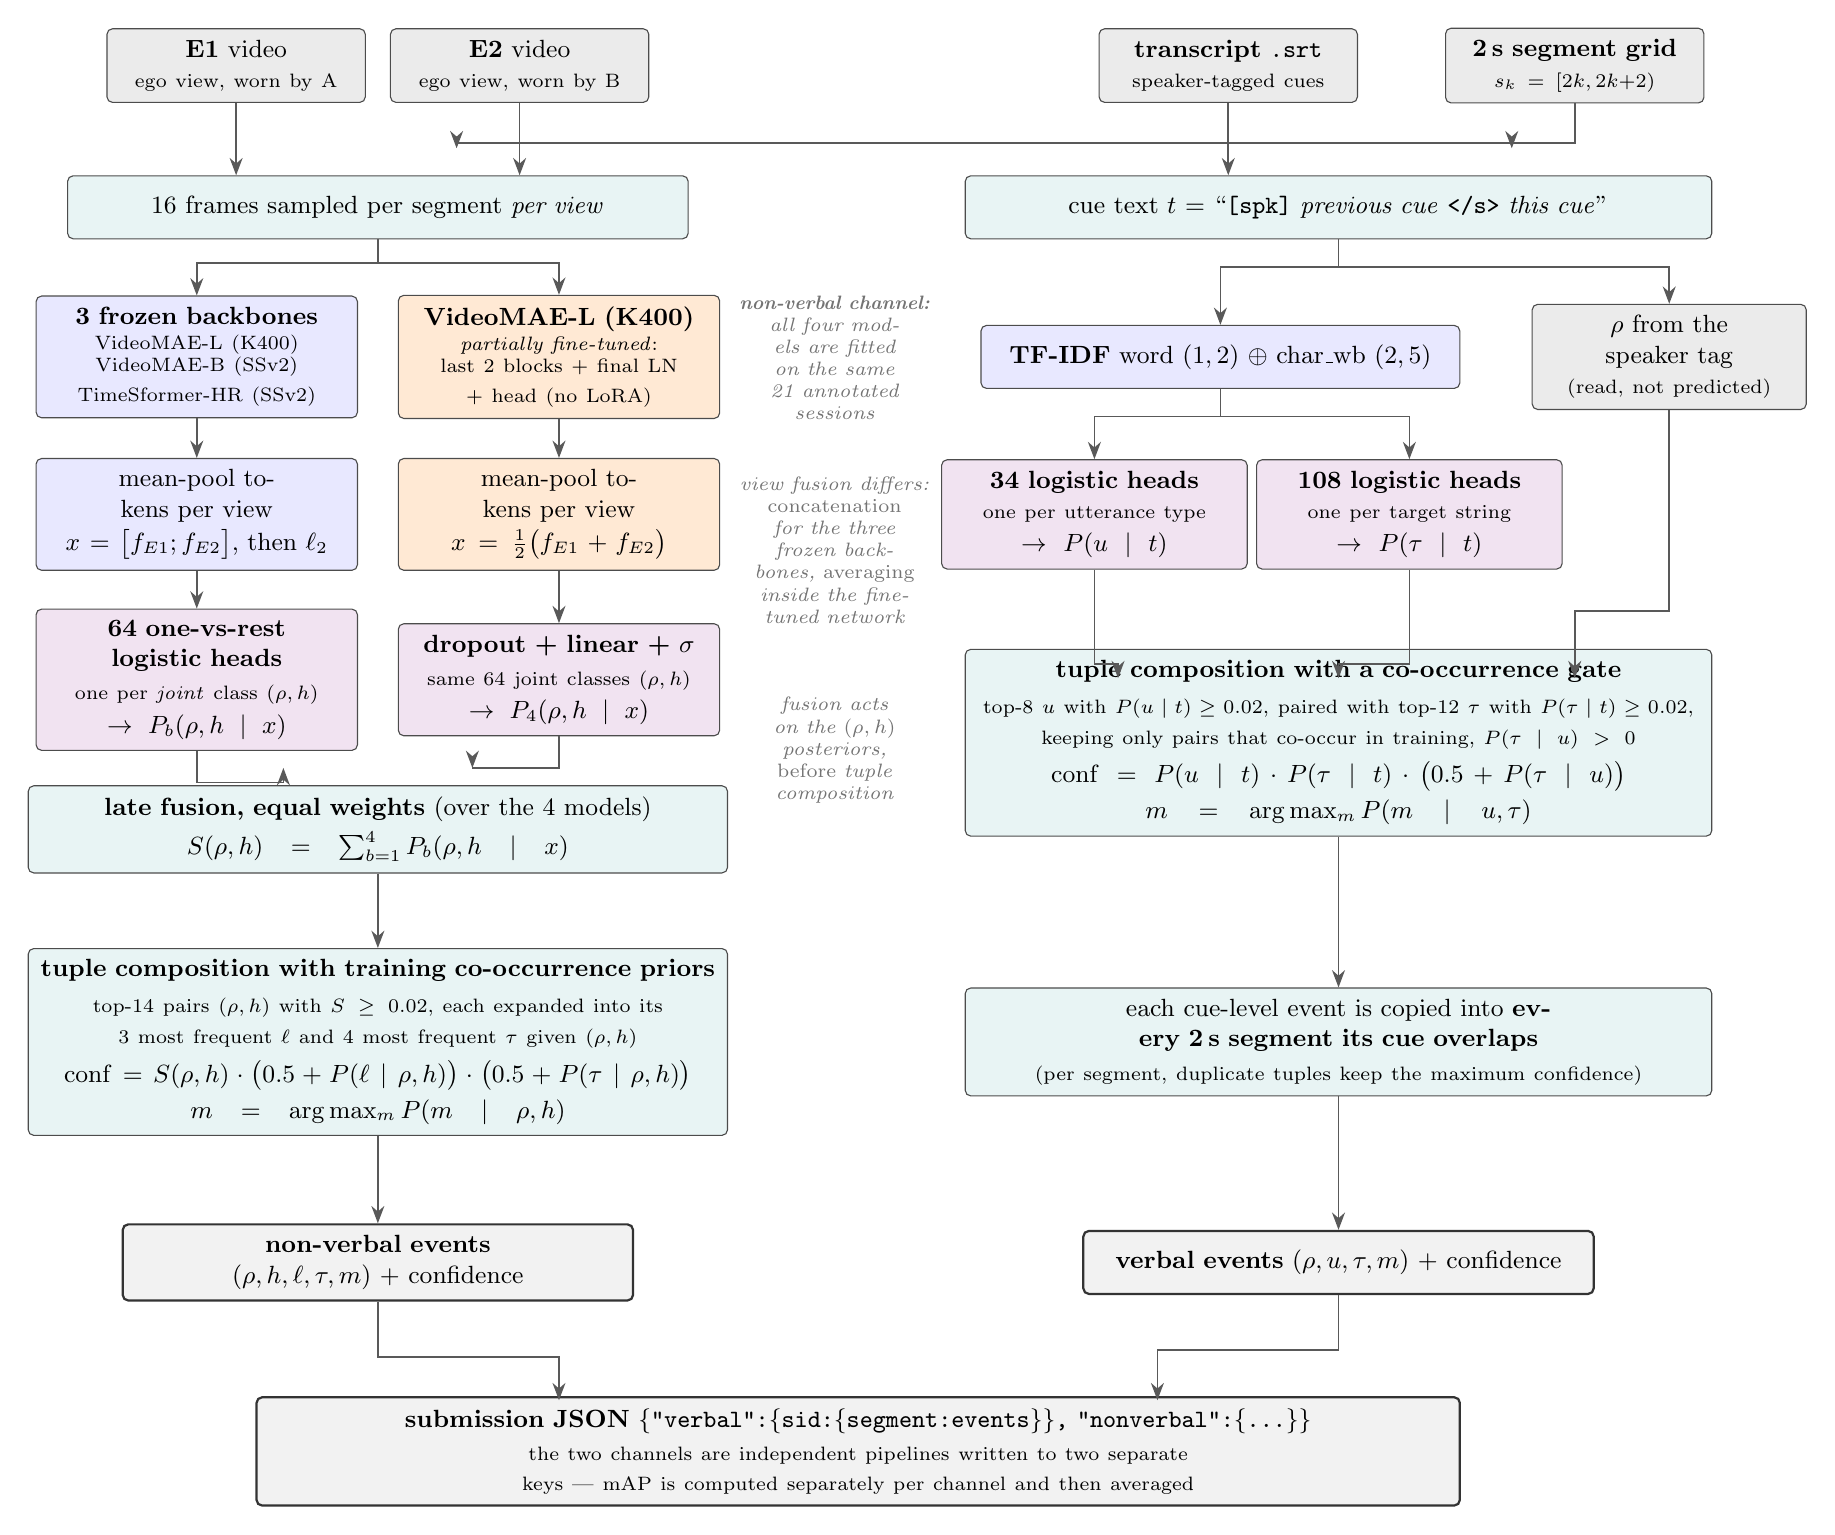
\begin{tikzpicture}[
  font=\small,
  >={Stealth[length=2.2mm]},
  box/.style     ={rounded corners=2pt, draw=black!70, align=center, inner sep=4pt,
                   minimum height=8mm, text width=#1},
  box/.default   =34mm,
  inp/.style     ={box=30mm, fill=black!8},
  enc/.style     ={box=38mm, fill=blue!9},
  ftb/.style     ={box=38mm, fill=orange!17},
  hd/.style      ={box=36mm, fill=violet!11},
  op/.style      ={box=86mm, fill=teal!9},
  outp/.style    ={box=38mm, fill=black!5, draw=black!80, thick},
  arr/.style     ={->, draw=black!65, semithick},
  note/.style    ={font=\scriptsize\itshape, text=black!55, align=center, text width=27mm}
]

% ================================================================ inputs
\node[inp] (e1)   at (-0.6,11.2) {\textbf{E1} video\\{\scriptsize ego view, worn by A}};
\node[inp] (e2)   at ( 3.0,11.2) {\textbf{E2} video\\{\scriptsize ego view, worn by B}};
\node[inp] (tr)   at (12.0,11.2) {\textbf{transcript} \texttt{.srt}\\{\scriptsize speaker-tagged cues}};
\node[inp] (grid) at (16.4,11.2) {\textbf{2\,s segment grid}\\{\scriptsize $s_k=[2k,2k{+}2)$}};

% ================================================================ non-verbal lane
\node[op, text width=76mm] (clip) at (1.2,9.4)
  {16 frames sampled per segment \emph{per view}};

\node[enc] (frozen) at (-1.1,7.5)
  {\textbf{3 frozen backbones}\\[1pt]
   {\scriptsize VideoMAE-L (K400)\\ VideoMAE-B (SSv2)\\ TimeSformer-HR (SSv2)}};
\node[ftb] (ftbb) at (3.5,7.5)
  {\textbf{VideoMAE-L (K400)}\\[1pt]
   {\scriptsize \emph{partially fine-tuned}:\\ last 2 blocks + final LN\\ + head (no LoRA)}};

\node[enc] (cat) at (-1.1,5.5)
  {mean-pool tokens per view\\[1pt] $x=\big[f_{E1};f_{E2}\big]$, then $\ell_2$};
\node[ftb] (avg) at (3.5,5.5)
  {mean-pool tokens per view\\[1pt] $x=\tfrac12\big(f_{E1}+f_{E2}\big)$};

\node[hd, text width=38mm] (lr) at (-1.1,3.4)
  {\textbf{64 one-vs-rest}\\\textbf{logistic heads}\\[1pt]
   {\scriptsize one per \emph{joint} class $(\rho,h)$}\\[1pt] $\rightarrow P_b(\rho,h\mid x)$};
\node[hd, text width=38mm] (fth) at (3.5,3.4)
  {\textbf{dropout + linear + $\sigma$}\\[1pt]
   {\scriptsize same 64 joint classes $(\rho,h)$}\\[1pt] $\rightarrow P_4(\rho,h\mid x)$};

\node[op] (fuse) at (1.2,1.5)
  {\textbf{late fusion, equal weights} (over the 4 models)\\[3pt]
   $S(\rho,h)=\sum_{b=1}^{4}P_b(\rho,h\mid x)$};

\node[op, minimum height=16mm] (compn) at (1.2,-1.2)
  {\textbf{tuple composition with training co-occurrence priors}\\[2pt]
   {\scriptsize top-14 pairs $(\rho,h)$ with $S\ge0.02$, each expanded into its}\\
   {\scriptsize 3 most frequent $\ell$ and 4 most frequent $\tau$ given $(\rho,h)$}\\[3pt]
   $\mathrm{conf}=S(\rho,h)\cdot\big(0.5+P(\ell\mid \rho,h)\big)\cdot\big(0.5+P(\tau\mid \rho,h)\big)$\\[2pt]
   $m=\arg\max\nolimits_m P(m\mid \rho,h)$};

\node[outp, text width=62mm] (outn) at (1.2,-4.0)
  {\textbf{non-verbal events} $(\rho,h,\ell,\tau,m)$ + confidence};

% ================================================================ verbal lane
\node[op, text width=92mm] (cue) at (13.4,9.4)
  {cue text $t$ = ``\texttt{[spk] }\emph{previous cue}\texttt{ </s> }\emph{this cue}''};

\node[enc, text width=58mm] (tfidf) at (11.9,7.5)
  {\textbf{TF-IDF} word $(1,2)$ $\oplus$ char\_wb $(2,5)$};
\node[inp, text width=32mm] (rho) at (17.6,7.5)
  {$\rho$ from the speaker tag\\{\scriptsize (read, not predicted)}};

\node[hd] (uh) at (10.3,5.5)
  {\textbf{34 logistic heads}\\{\scriptsize one per utterance type}\\[1pt] $\rightarrow P(u\mid t)$};
\node[hd] (th) at (14.3,5.5)
  {\textbf{108 logistic heads}\\{\scriptsize one per target string}\\[1pt] $\rightarrow P(\tau\mid t)$};

\node[op, text width=92mm, minimum height=16mm] (compv) at (13.4,2.6)
  {\textbf{tuple composition with a co-occurrence gate}\\[2pt]
   {\scriptsize top-8 $u$ with $P(u\mid t)\ge0.02$, paired with top-12 $\tau$ with $P(\tau\mid t)\ge0.02$,}\\
   {\scriptsize keeping only pairs that co-occur in training, $P(\tau\mid u)>0$}\\[3pt]
   $\mathrm{conf}=P(u\mid t)\cdot P(\tau\mid t)\cdot\big(0.5+P(\tau\mid u)\big)$\\[2pt]
   $m=\arg\max\nolimits_m P(m\mid u,\tau)$};

\node[op, text width=92mm] (assign) at (13.4,-1.2)
  {each cue-level event is copied into \textbf{every 2\,s segment its cue overlaps}\\[1pt]
   {\scriptsize (per segment, duplicate tuples keep the maximum confidence)}};

\node[outp, text width=62mm] (outv) at (13.4,-4.0)
  {\textbf{verbal events} $(\rho,u,\tau,m)$ + confidence};

% ================================================================ output
\node[outp, text width=150mm, minimum height=11mm] (json) at (7.3,-6.4)
  {\textbf{submission JSON} \texttt{\{"verbal":\{sid:\{segment:events\}\},\ "nonverbal":\{\dots\}\}}\\[1pt]
   {\scriptsize the two channels are independent pipelines written to two separate keys ---
    mAP is computed separately per channel and then averaged}};

% ================================================================ arrows
\draw[arr] (e1) -- (e1|-clip.north);
\draw[arr] (e2) -- (e2|-clip.north);
\draw[arr] (tr) -- (tr|-cue.north);
\draw[arr] (grid.south) -- ++(0,-0.5) -| (2.2,10.15);
\draw[arr] (grid.south) -- ++(0,-0.5) -| (15.6,10.15);

\draw[arr] (clip.south) -- ++(0,-0.3) -| (frozen.north);
\draw[arr] (clip.south) -- ++(0,-0.3) -| (ftbb.north);
\draw[arr] (frozen) -- (cat);
\draw[arr] (ftbb) -- (avg);
\draw[arr] (cat) -- (lr);
\draw[arr] (avg) -- (fth);
\draw[arr] (lr.south) -- ++(0,-0.4) -| (0.0,2.28);
\draw[arr] (fth.south) -- ++(0,-0.4) -| (2.4,2.28);
\draw[arr] (fuse) -- (compn);
\draw[arr] (compn) -- (outn);

\draw[arr] (cue.south) -- ++(0,-0.35) -| (tfidf.north);
\draw[arr] (cue.south) -- ++(0,-0.35) -| (rho.north);
\draw[arr] (tfidf.south) -- ++(0,-0.35) -| (uh.north);
\draw[arr] (tfidf.south) -- ++(0,-0.35) -| (th.north);
\draw[arr] (uh.south) -- ++(0,-1.2) -| (10.6,3.42);
\draw[arr] (th.south) -- ++(0,-1.2) -| (13.4,3.42);
\draw[arr] (rho.south) -- ++(0,-2.55) -| (16.4,3.42);
\draw[arr] (compv) -- (assign);
\draw[arr] (assign) -- (outv);

\draw[arr] (outn.south) -- ++(0,-0.7) -| (3.5,-5.75);
\draw[arr] (outv.south) -- ++(0,-0.7) -| (11.1,-5.75);

% ================================================================ margin notes (in the gutter)
\node[note, anchor=north] at (7.0,8.4)
  {\textbf{non-verbal channel:}\\ all four models are fitted\\ on the same 21 annotated\\ sessions};
\node[note, anchor=north] at (7.0,6.1)
  {view fusion differs:\\ \emph{concatenation} for the three\\ frozen backbones,
   \emph{averaging}\\ inside the fine-tuned network};
\node[note, anchor=north] at (7.0,3.3)
  {fusion acts on the $(\rho,h)$\\ posteriors, \emph{before} tuple\\ composition};
\end{tikzpicture}
\end{document}
